\documentclass{article}
\usepackage[utf8]{inputenc}
\usepackage[russian]{babel}
\usepackage{graphicx}
\usepackage{amsmath}
\usepackage{breqn}
\usepackage{wrapfig}
\usepackage{float}
\usepackage{multirow}
\usepackage{caption}
\usepackage{subcaption}

\graphicspath{ {./data/images} }
\author{Александр Романов Б01-107}
\date{}
\title{4.3.5 Изучение голограммы}

\begin{document}
\maketitle
\section{Введение}
\subsection{Цель работы}
Изучить свойства голограмм точечного источника и объёмного предмета.
\subsection{В работе используются}
Гелий-неоновый лазер, голограммы, набор линз, предметная шкала, экран, линейка.
\begin{figure}[H]
  \centering
  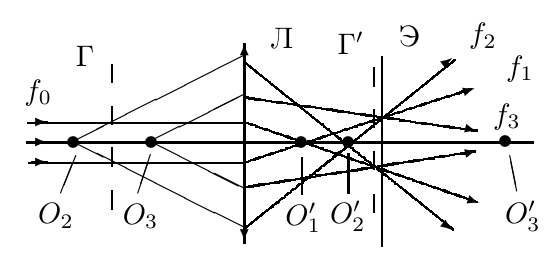
\includegraphics[width=\textwidth]{scheme.png}
  \caption{Схема установки}
\end{figure}
\section{Работа}

\subsection{А. Изучение характеристик голограммы точечного источника.}
В этом пункте предлагается рассчитать расстояние от голограммы до точечного источника, который использовался при её создании:
\begin{enumerate}
  \item По результатам измерения радиуса голографических колкц, спроектированных на удалённый экран при помощи
  короткофокусной линзы
  \item По результатам измерения параметров проекционной установки, в которой голограмма используется как фокусирующая линза, а объектом
  служит предметная шкала.
\end{enumerate}

\subsubsection{Определение цены деления}
Включим лазер. Для определения цены деления предметной шкалы установим кассету с транспарантами вблизи лазера.
Осветим лазером шкалу и получим на удалённом экране дифракционную картину, созданную крестообразной шкалой.

Определив расстояние \(\Delta x\) между дифракционными максимума на экране и расстояние \(L\) от шкалы до
экрана, рассчитаем цену деления \(D\) по извеснтой формуле для дифракции Фраунгофера:
\[\frac{\lambda}{D} = \frac{\Delta x}{L}\]
\[\Delta x = (5.50 \pm 0.05)\;mm\]
\[L = (114.0pm0.1)\; cm\]
\[\lambda = 532\; nm\]
Отсюда:
\[D = \frac{\lambda L}{\Delta x} = (0.11 \pm 0.01)\; mm\]

Определим цену деления той же шкалы, используя линзу с фокусным расстоянием \(F \simeq 4\;cm\).
Получим в центре экрана увеличенное изображение предметной шкалы с чёткими делениями.

Измерим расстояния от линзы до предметной шкалы \((a = (6.5\pm0.1)\; cm)\) и до экрана \((b = (107.5\pm 0.1)\;cm)\).
Расттояние между делениями на экране (\(D' = (2.0 \pm 0.2)\; mm \)).
Рассчитаем увеличение системы и цену деления \(D\):
\[ D = \frac{D'}{b/a} = (0.12\pm0.01)\;mm \]

Результаты, полученные обоими способами, совпадают в пределах погрешности. Первый результат должен быть точнее, т.к. погрешность
длины волны лазера должна быть меньше чем погрешность фокусного расстояния.

\subsubsection{Определение расстояния от голограммы до точечного источника}
Осветим Лазером окно №2 с голограммой. Увидим на экране 3 световых пятна. Перемещая голограмму по вертикали, добъёмся того, чтобы
все 3 пятна были на одной высоте. Совместив все 3 пятна получим изображение голограммы (набор концентрических колец).
Приложим к экрану лист бумаги и отметим на нём радиус второго светлого кольца (\( r_2' = (3.5 \pm 0.5)\; mm\)).
Измерим расстояния от линзы до предметной шкалы \((a = (5.30\pm0.05)\; cm)\) и до экрана \((b = (108.7\pm 0.05)\;cm)\).
Расчитаем размеры колец на голограмме:
\[r_2 = \frac{r_2'}{b/a} = (0.17 \pm 0.05)\; mm\]
Теперь расчитаем расстояние от голограммы до точечного источника:
\[ r_m = \sqrt{m\lambda d} \Rightarrow d = \frac{r_2^2}{m\lambda} = (2.7\pm0.3)\; cm\]

Перемещая линзу вдоль луча, получите на экране изображение сначала мнимого \(O_2\), а затем действительного точечного
источника \(O_3\). Для каждого изображения рассчитаем расстояния от точечного источника до голограммы:
\[ d_2 = (3.2 \pm 0.3)\; cm \]
\[ d_3 = (3.3 \pm 0.3)\; cm \]

\subsubsection{Изучение фокусиркющих свойств голограммы}
В этом опыте сама голограммы выполняет роль короткофокусной линзы. В качестве траспаранта, увеличенное изображение которого
требуется получить с помощью голографической линзы, используется предметная шкала, закреплённая в отдельной оправе.

Сначала неболшим перемещением голограммы по вертикали и вращением вокруг вертикальной оси добъёмся полного разделения пучков света
на удалённом экране. 

Установим переносной экран на расстоянии \(\simeq 50\; cm\) за голограммой. Перед голограммой (вплотную к ней)
поставим предметную шкалу, закреплённую в отдельной оправе. Отодвигая рейтер со шкалой от голограммы,
получим в одном из пятен резкое изображение делений крестообразной шкалы.

Измерьте расстояние между штрихами (\(D' = (0.56\pm0.01)\; cm\)) на экране и расстояние \(b = (113.50 \pm 0.05\; cm)\) от экрана до голограммы.
Используя эти данные, а также найденную ранее цену деления \(D\), рассчитаем расстояние от линзы до предмета:
\[\frac{b}{a} = \frac{D'}{D} \Rightarrow a = \frac{b}{D'/D} = (2.3\pm0.1)\;cm\]

\subsection{Б. Изучение характеристик голограммы объёмного предмета}
\subsubsection{Юстировка системы}
Учтановим линзу с фокусным расстоянием \(\simeq 9\;cm\) на расстояние \(\simeq 50\; cm\) от экрана. И, перемещая линзу
в плоскости, перпендикулярной оптической оси, совместим центр светового пятна с точкой, где распологалось пятно в отсутствии линзы.

На расстоянии \(\simeq 10\;cm\) перед длиннофокусной линзой установим короткофокусную линзу с \(f = 2\;mm\). Перемещая короткофокусную
линзу в плоскости перпендикулярной лучу, вновь совместим центр светового пятна с его начальным положением.

Перемещением короткофокусной линзы, добъёмся того, чтобы из собранного расширителя выходил параллельный пучок.

\subsubsection{Изучение мнимого изображения}
Поместим голограмму в расширенный пучок лазера фотоэмульсией к лазеру и найдём мнимое изображение предмета. Изображение на самом деле объёмное.
При перемещении глаза изменяется перспектива.

\begin{figure}[H]
  \centering
  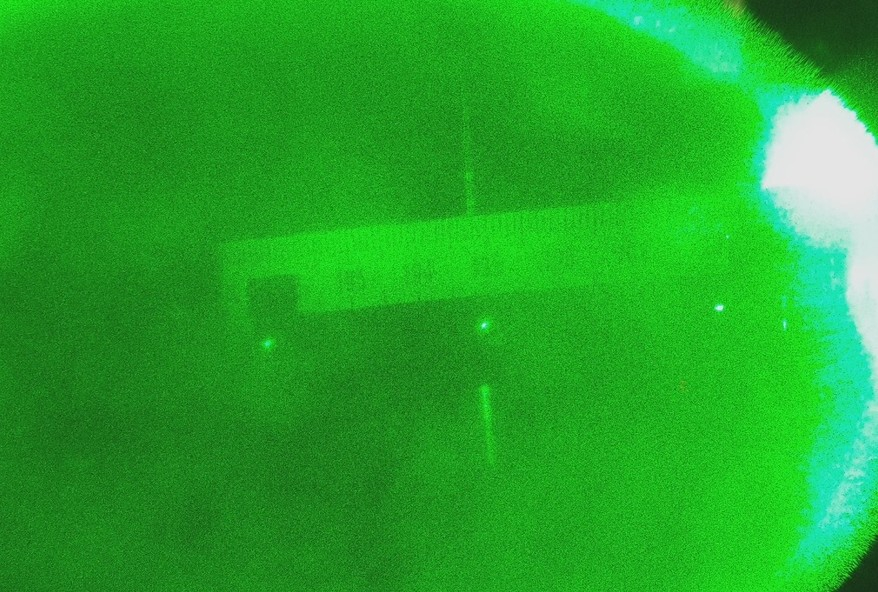
\includegraphics[width=\textwidth]{image.jpg}
  \caption{Наблюдаемое мнимое изображение}
\end{figure}

По углу поворота голограммы оценим угол падения опорной волны, который был выбран при получении голограммы:
\[ \alpha = 45^\circ \]

\subsubsection{Изучение действительного изображения}
Расположим голограмму перпендикулярно падающему пучку света, наблюдать будем с левой стороны. Повернём голограмму фотоэмульсией от лазера и пронаблюдаем
изображения. Они зеркальны предыдущим.


\section{Выводы}
В ходе выполнения работы:
\begin{enumerate}
  \item \[ d_2 = (3.2 \pm 0.3)\; cm \]
\[ d_3 = (3.3 \pm 0.3)\; cm \]Были изучены свойства голограмм точечного источника и предмета.
  \item Были разными способами посчитаны цены деления предметной шкалы. Эти значения:
  \[(0.11 \pm 0.01)\; mm\;\; \text{vs}\;\;  (0.12\pm0.01)\;mm\]
  Совпадают в пределах погрешности.
  \item Было измерено расстояние от голограммы до точечного источника до голограммы:
  \[d= (2.7\pm0.3)\; cm\]
  Расстояния от мнимого и действительного источников до голограммы:
  \[ d_2 = (3.2 \pm 0.3)\; cm \]
  \[ d_3 = (3.3 \pm 0.3)\; cm \]
  \item Были изученны фокусирующие свойства диаграммы и найдено расстояние от линзы до предмета:
  \[a = (2.3\pm0.1)\;cm\]
  Это значение близко к реальности.
  \item Было получено изображение голограммы объёмного предмета.
\end{enumerate}
\end{document}